\sectionname{Computer Modern}

Various companies have created Type~1 versions of the Computer Modern fonts;
those versions can be run through MathGen just as easily as any other Type~1
font. Comparison of the generated parameters with those of Computer Modern
reveal that MathGen has successfully captured, with good accuracy, the
parameters of Computer Modern.

\begin{figure*}
\begin{center}
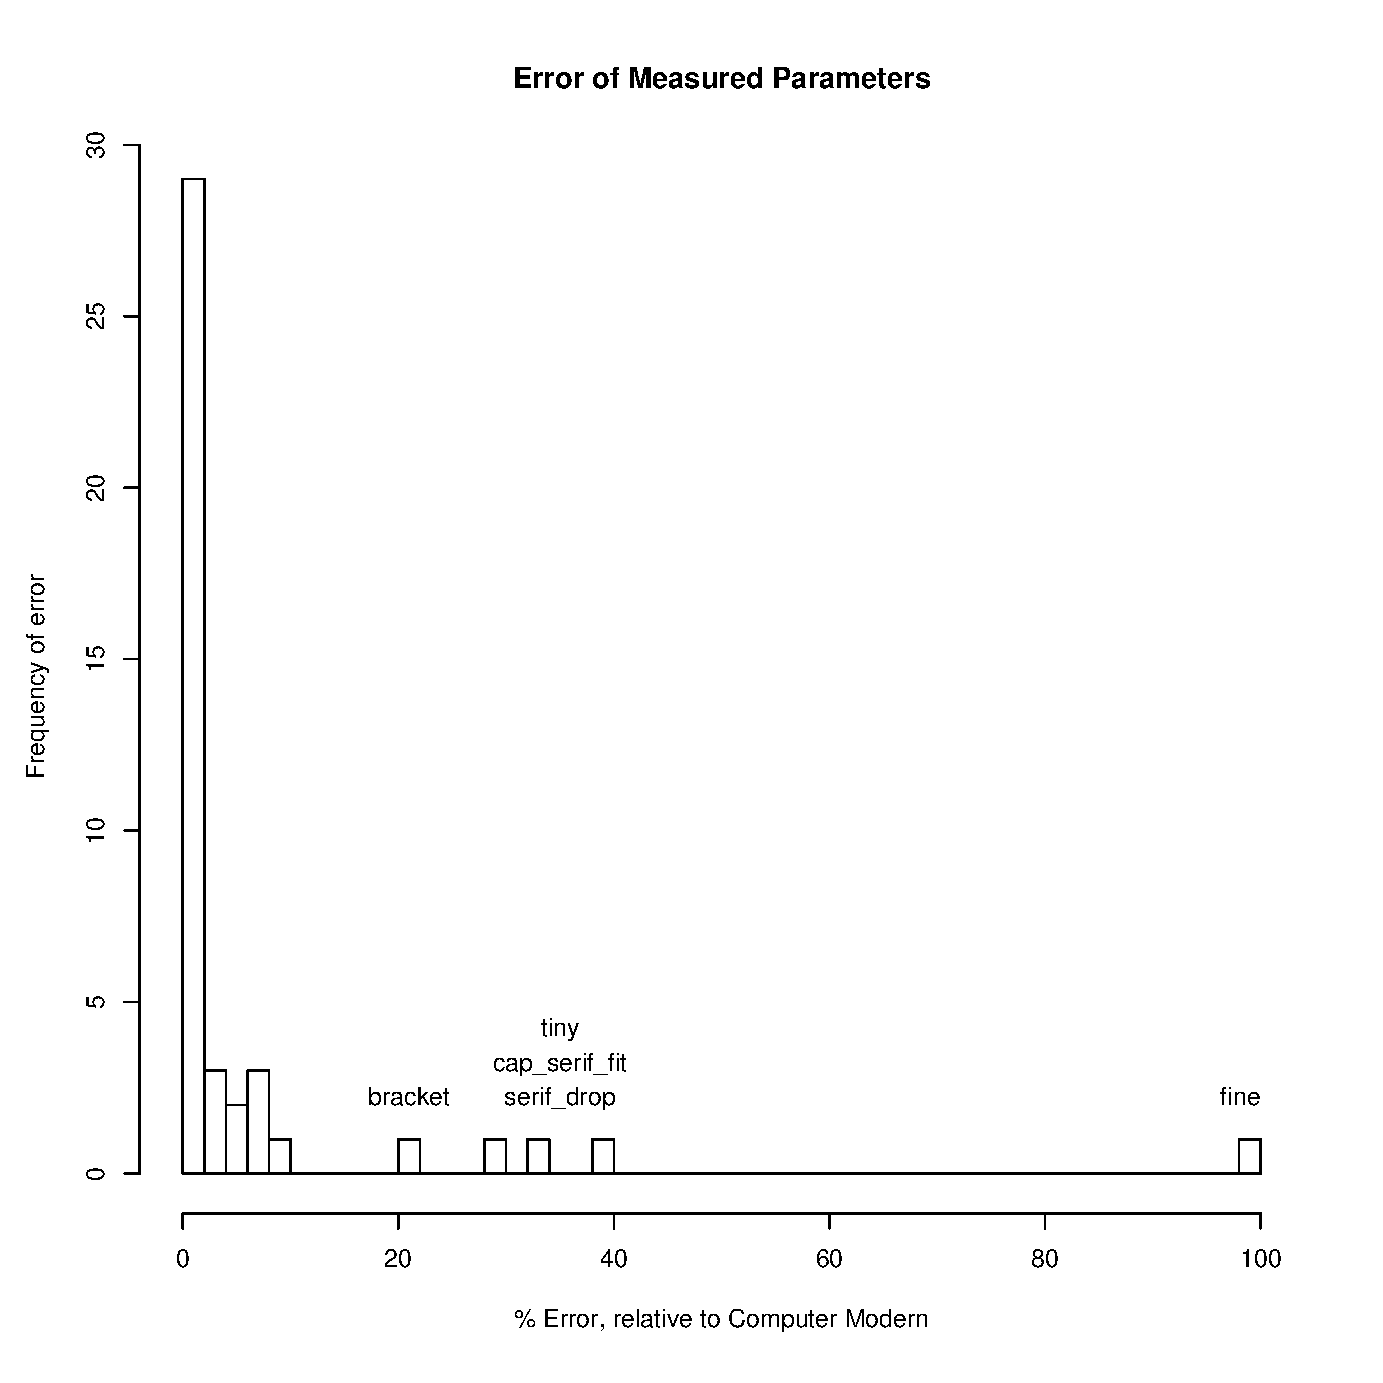
\includegraphics[width=6in]{params/cmr}
\end{center}
\caption{Histogram of the relative errors of the measured parameters of the
Computer Modern font, calculated by the percent difference between the original
value and the measured one.}
\label{f:cmr}
\end{figure*}

Figure~\ref{f:cmr} shows the percent error of the measured parameters, compared
against the original parameters of Computer Modern. As the graph shows, most of
the parameters are measured within a few percent accuracy. The four main
outliers are named there. The outliers are as follows:
\begin{itemize}
\item The \emph{fine} and \emph{tiny} parameters define the curvatures around
very small corners; their values change the stylistic appearance of the math
fonts but not compatibility with the text.
\item The \emph{cap\_serif\_fit} parameter measures the amount of extra space
surrounding the $\Pi$, $\Gamma$, and $\Lambda$ characters. Currently that
parameter is chosen in a somewhat ad-hoc fashion; further improvements could
make that value more accurate.\looseness=-1
\item The \emph{serif\_drop} parameter measures the amount by which serifs at
the tops of letters (i, l) are slanted. It is unfortunate that this value is so
incorrect for Computer Modern (it is more accurate for nearly every other font
tested), but it is not too significant, as it only affects one generated letter
($\nu$).
\item The \emph{bracket} parameter measures the amount of curvature between a
horizontal serif and the upward stem. It turns out that, because of the way
serifs are drawn, the error will be divided by three, so it is not terribly
worrisome. Additionally, serif bracket tends to be somewhat fickle to measure,
but as long as a reasonable value is chosen, the serif will look correct.
\end{itemize}
We can also calculate error relative to the font's overall size. In that case,
practically all the measurement errors are below 1\%; the only substantial
exception being the parameter \emph{fig\_height}, which is never used in
MathGen.
